\documentclass{standalone}
\usepackage{tikz}
\usepackage{ctex,siunitx}
\setCJKmainfont{Noto Serif CJK SC}
\usepackage{tkz-euclide}
\usepackage{amsmath}
\usetikzlibrary{patterns, calc,3d}
\usetikzlibrary {decorations.pathmorphing,decorations.pathreplacing,decorations.shapes}
\begin{document}
\small
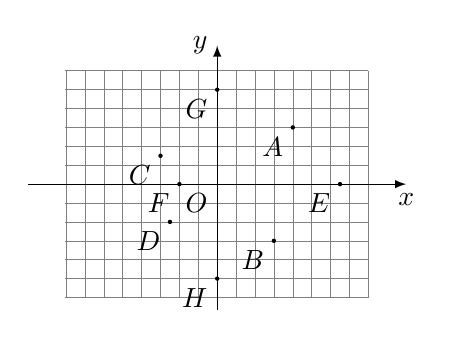
\begin{tikzpicture}[>=latex,scale=0.8]
  \draw[help lines,gray,very thin, step=3mm](-2.41,-1.8)grid(2.4,1.8);
  \draw[->](-3,0)--(3,0)node[below]{$x$};
  \draw[->](0,-2.0)--(0,2.2)node[left]{$y$};
  \node at (0,0)[below left]{$O$};
  \foreach \x/\y/\t in {
    4/3/A,
    3/-3/B,
    -3/1.5/C,
    -2.5/-2/D,
    6.5/0/E,
    -2/0/F,
    0/5/G,
    0/-5/H
  }
  {
    \fill(0.3*\x,0.3*\y)circle(1pt)node[below left]{$\t$};
  }
\end{tikzpicture}
\end{document}